% Options for packages loaded elsewhere
\PassOptionsToPackage{unicode}{hyperref}
\PassOptionsToPackage{hyphens}{url}
%
\documentclass[
  man,floatsintext]{apa6}
\usepackage{amsmath,amssymb}
\usepackage{lmodern}
\usepackage{iftex}
\ifPDFTeX
  \usepackage[T1]{fontenc}
  \usepackage[utf8]{inputenc}
  \usepackage{textcomp} % provide euro and other symbols
\else % if luatex or xetex
  \usepackage{unicode-math}
  \defaultfontfeatures{Scale=MatchLowercase}
  \defaultfontfeatures[\rmfamily]{Ligatures=TeX,Scale=1}
\fi
% Use upquote if available, for straight quotes in verbatim environments
\IfFileExists{upquote.sty}{\usepackage{upquote}}{}
\IfFileExists{microtype.sty}{% use microtype if available
  \usepackage[]{microtype}
  \UseMicrotypeSet[protrusion]{basicmath} % disable protrusion for tt fonts
}{}
\makeatletter
\@ifundefined{KOMAClassName}{% if non-KOMA class
  \IfFileExists{parskip.sty}{%
    \usepackage{parskip}
  }{% else
    \setlength{\parindent}{0pt}
    \setlength{\parskip}{6pt plus 2pt minus 1pt}}
}{% if KOMA class
  \KOMAoptions{parskip=half}}
\makeatother
\usepackage{xcolor}
\usepackage{graphicx}
\makeatletter
\def\maxwidth{\ifdim\Gin@nat@width>\linewidth\linewidth\else\Gin@nat@width\fi}
\def\maxheight{\ifdim\Gin@nat@height>\textheight\textheight\else\Gin@nat@height\fi}
\makeatother
% Scale images if necessary, so that they will not overflow the page
% margins by default, and it is still possible to overwrite the defaults
% using explicit options in \includegraphics[width, height, ...]{}
\setkeys{Gin}{width=\maxwidth,height=\maxheight,keepaspectratio}
% Set default figure placement to htbp
\makeatletter
\def\fps@figure{htbp}
\makeatother
\setlength{\emergencystretch}{3em} % prevent overfull lines
\providecommand{\tightlist}{%
  \setlength{\itemsep}{0pt}\setlength{\parskip}{0pt}}
\setcounter{secnumdepth}{-\maxdimen} % remove section numbering
% Make \paragraph and \subparagraph free-standing
\ifx\paragraph\undefined\else
  \let\oldparagraph\paragraph
  \renewcommand{\paragraph}[1]{\oldparagraph{#1}\mbox{}}
\fi
\ifx\subparagraph\undefined\else
  \let\oldsubparagraph\subparagraph
  \renewcommand{\subparagraph}[1]{\oldsubparagraph{#1}\mbox{}}
\fi
\newlength{\cslhangindent}
\setlength{\cslhangindent}{1.5em}
\newlength{\csllabelwidth}
\setlength{\csllabelwidth}{3em}
\newlength{\cslentryspacingunit} % times entry-spacing
\setlength{\cslentryspacingunit}{\parskip}
\newenvironment{CSLReferences}[2] % #1 hanging-ident, #2 entry spacing
 {% don't indent paragraphs
  \setlength{\parindent}{0pt}
  % turn on hanging indent if param 1 is 1
  \ifodd #1
  \let\oldpar\par
  \def\par{\hangindent=\cslhangindent\oldpar}
  \fi
  % set entry spacing
  \setlength{\parskip}{#2\cslentryspacingunit}
 }%
 {}
\usepackage{calc}
\newcommand{\CSLBlock}[1]{#1\hfill\break}
\newcommand{\CSLLeftMargin}[1]{\parbox[t]{\csllabelwidth}{#1}}
\newcommand{\CSLRightInline}[1]{\parbox[t]{\linewidth - \csllabelwidth}{#1}\break}
\newcommand{\CSLIndent}[1]{\hspace{\cslhangindent}#1}
\ifLuaTeX
\usepackage[bidi=basic]{babel}
\else
\usepackage[bidi=default]{babel}
\fi
\babelprovide[main,import]{english}
% get rid of language-specific shorthands (see #6817):
\let\LanguageShortHands\languageshorthands
\def\languageshorthands#1{}
% Manuscript styling
\usepackage{upgreek}
\captionsetup{font=singlespacing,justification=justified}

% Table formatting
\usepackage{longtable}
\usepackage{lscape}
% \usepackage[counterclockwise]{rotating}   % Landscape page setup for large tables
\usepackage{multirow}		% Table styling
\usepackage{tabularx}		% Control Column width
\usepackage[flushleft]{threeparttable}	% Allows for three part tables with a specified notes section
\usepackage{threeparttablex}            % Lets threeparttable work with longtable

% Create new environments so endfloat can handle them
% \newenvironment{ltable}
%   {\begin{landscape}\centering\begin{threeparttable}}
%   {\end{threeparttable}\end{landscape}}
\newenvironment{lltable}{\begin{landscape}\centering\begin{ThreePartTable}}{\end{ThreePartTable}\end{landscape}}

% Enables adjusting longtable caption width to table width
% Solution found at http://golatex.de/longtable-mit-caption-so-breit-wie-die-tabelle-t15767.html
\makeatletter
\newcommand\LastLTentrywidth{1em}
\newlength\longtablewidth
\setlength{\longtablewidth}{1in}
\newcommand{\getlongtablewidth}{\begingroup \ifcsname LT@\roman{LT@tables}\endcsname \global\longtablewidth=0pt \renewcommand{\LT@entry}[2]{\global\advance\longtablewidth by ##2\relax\gdef\LastLTentrywidth{##2}}\@nameuse{LT@\roman{LT@tables}} \fi \endgroup}

% \setlength{\parindent}{0.5in}
% \setlength{\parskip}{0pt plus 0pt minus 0pt}

% Overwrite redefinition of paragraph and subparagraph by the default LaTeX template
% See https://github.com/crsh/papaja/issues/292
\makeatletter
\renewcommand{\paragraph}{\@startsection{paragraph}{4}{\parindent}%
  {0\baselineskip \@plus 0.2ex \@minus 0.2ex}%
  {-1em}%
  {\normalfont\normalsize\bfseries\itshape\typesectitle}}

\renewcommand{\subparagraph}[1]{\@startsection{subparagraph}{5}{1em}%
  {0\baselineskip \@plus 0.2ex \@minus 0.2ex}%
  {-\z@\relax}%
  {\normalfont\normalsize\itshape\hspace{\parindent}{#1}\textit{\addperi}}{\relax}}
\makeatother

% \usepackage{etoolbox}
\makeatletter
\patchcmd{\HyOrg@maketitle}
  {\section{\normalfont\normalsize\abstractname}}
  {\section*{\normalfont\normalsize\abstractname}}
  {}{\typeout{Failed to patch abstract.}}
\patchcmd{\HyOrg@maketitle}
  {\section{\protect\normalfont{\@title}}}
  {\section*{\protect\normalfont{\@title}}}
  {}{\typeout{Failed to patch title.}}
\makeatother

\usepackage{xpatch}
\makeatletter
\xapptocmd\appendix
  {\xapptocmd\section
    {\addcontentsline{toc}{section}{\appendixname\ifoneappendix\else~\theappendix\fi\\: #1}}
    {}{\InnerPatchFailed}%
  }
{}{\PatchFailed}
\keywords{learning, R, statistical programming, error-full learning\newline\indent Word count: 1018}
\usepackage{lineno}

\linenumbers
\usepackage{csquotes}
\ifLuaTeX
  \usepackage{selnolig}  % disable illegal ligatures
\fi
\IfFileExists{bookmark.sty}{\usepackage{bookmark}}{\usepackage{hyperref}}
\IfFileExists{xurl.sty}{\usepackage{xurl}}{} % add URL line breaks if available
\urlstyle{same} % disable monospaced font for URLs
\hypersetup{
  pdftitle={The effect of erroneous R code on developing data skills},
  pdfauthor={James Bartlett1},
  pdflang={en-EN},
  pdfkeywords={learning, R, statistical programming, error-full learning},
  hidelinks,
  pdfcreator={LaTeX via pandoc}}

\title{The effect of erroneous R code on developing data skills}
\author{James Bartlett\textsuperscript{1}}
\date{}


\shorttitle{Erroneous R code}

\authornote{

This demonstration is based on mock data.

The authors made the following contributions. James Bartlett: Conceptualization, Writing - Original Draft Preparation, Writing - Review \& Editing.

Correspondence concerning this article should be addressed to James Bartlett, 62 Hillhead Street, Glasgow. E-mail: \href{mailto:james.bartlett@glasgow.ac.uk}{\nolinkurl{james.bartlett@glasgow.ac.uk}}

}

\affiliation{\vspace{0.5cm}\textsuperscript{1} University of Glasgow, United Kingdom}

\abstract{%
Teaching statistical programming languages like R are key for adopting reproducible data preparation and analysis workflows. However, teaching data skills provides unique challenges such as preparing students to debug coding errors.

We randomly allocated students to complete an error-free (n = 145) or error-full (n = 130) version of a lecture, to investigate if teaching debugging skills improves students performance on a data skills assignment.

Students in the error-full lecture performed significantly better on the data skills assignment than students in the error-free lecture, with a mean improvement of 4.94\%, 95\% CI {[}2.40, 7.49{]}.

Adopting a lecture format that covers both data wrangling and debugging skills has the potential to improve student's understanding of reproducible data preparation and analysis.
}



\begin{document}
\maketitle

Data skills are increasingly recognised as a key component of psychological literacy. To promote reproducible data preparation and analysis workflows, educators have highlighted the role of teaching students how to use statistical programming languages instead of point-and-click software (McAleer et al., 2022). However, programming is rare in UK psychology curricula (TARG Meta-Research Group, 2022) and offers unique challenges such as how to prepare students to debug their code. Debugging code is a separate problem solving skill to learn alongside statistics, so it is important to understand how best to teach students debugging skills.

Hoffman and Elmi (2021) reported a small pilot study using SAS where they compared a traditional error-free course structure to an error-full course focusing on debugging errors alongside key concepts. 80\% of students preferred the error-full course but the study only included 18 participants and just 4 students completed assignments following each course, meaning they could not compare performance. Therefore, in our study, we want to apply these methods to the programming language R and recruit a larger sample.

We hypothesise that students who complete the error-full lecture will score higher on a data skills assignment than students who complete the error-free lecture.

\hypertarget{methods}{%
\section{Methods}\label{methods}}

\hypertarget{participants}{%
\subsection{Participants}\label{participants}}

Before collecting data, we performed an \emph{a priori} power analysis to calculate how many participants we would need. Hoffman and Elmi (2021) did not report any performance data, so we used Bebermeier and Hagemann (2019) to set our smallest effect size of interest. They investigated the effect of creating statistics exercises based on research article. The researchers found students performed better on a class assignment when they completed these exercises than when students did not complete the exercises (\emph{d} = 0.55). The authors did not comment on the effect size, so we chose a more conservative estimate based on the small telescopes approach (Simonsohn, 2015) for the effect size the original study had 33\% power to detect. Using an effect size of d = 0.38, we aimed to recruit 149 participants per group for an independent samples t-test (\(\alpha\) = 0.05, power = 0.90).

We finished with two groups of 145 and 130 participants (N = 275), slightly fewer than our initial target.

\hypertarget{material}{%
\subsection{Material}\label{material}}

In the error-free lecture, students heard a one hour presentation on data wrangling, showing how to use Tidyverse functions like mutate, filter, and select.

In the error-full lecture, students heard a one hour presentation on data wrangling, the same as in the error-free group. However, in this group we also guided students through an error interpretation session to demonstrate common errors when using these data wrangling functions.

Both groups of students completed the same data skills assignment on data wrangling where students had to write code to solve problems and debug errors. Scores could range from 0-100\%.

\hypertarget{procedure}{%
\subsection{Procedure}\label{procedure}}

We offered participants an additional bonus lecture outside their normal course curriculum. Students could register interest on their course page and provide informed consent. On sign up, students were randomly allocated to attend the error-free lecture or error-full lecture. In the hour immediately following the lecture, students completed the data skills assignment and were debriefed. We provided students who did not receive the error-full lecture a link to the lecture recording to ensure they received the debugging guidance. We demonstrate the procedure as a diagram in Figure \ref{fig:procedure-diagram}.



\begin{figure}
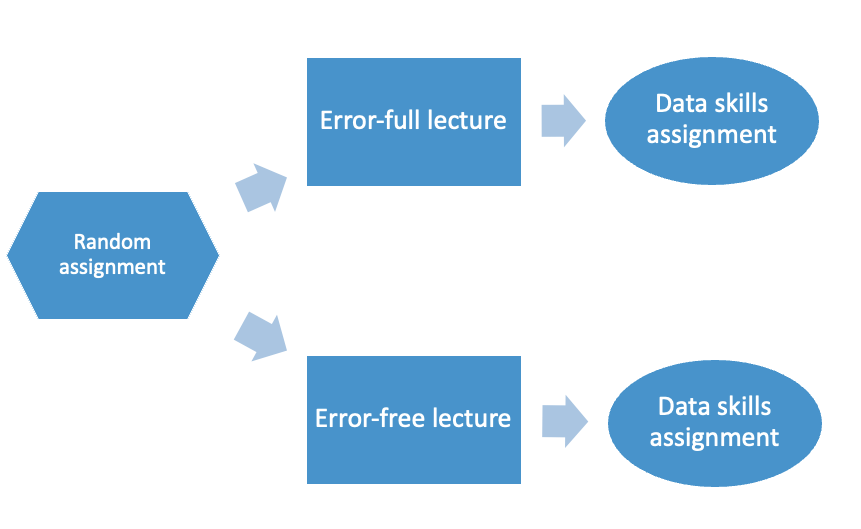
\includegraphics[width=1\linewidth]{Figures/procedure_diagram} \caption{Procedure diagram showing how students were randomly allocated to an error-free or error-full version of a lecture before completing a data skills assignment.}\label{fig:procedure-diagram}
\end{figure}

\hypertarget{design-and-data-analysis}{%
\subsection{Design and data analysis}\label{design-and-data-analysis}}

We had one between-subjects IV with two levels. Participants were randomly allocated to attend the error-free (level 1) or error-full (level 2) version of the lecture. We had one dependent variable of their score on the data skills assignment which could range between 0-100\%.

Data met parametric assumptions and we used a Welch t-test to compare the two groups on their data skills score. We used a two-tailed test as we expected the error-full lecture to produce higher scores, but we were open to the possibility that the error-free lecture could produce higher scores.

\hypertarget{results}{%
\section{Results}\label{results}}

\begin{table}[tbp]

\begin{center}
\begin{threeparttable}

\caption{\label{tab:descriptives-table}Descriptive statistics of data skills assignment for each lecture group.}

\begin{tabular}{lllll}
\toprule
Group & \multicolumn{1}{c}{Mean} & \multicolumn{1}{c}{SD} & \multicolumn{1}{c}{Min} & \multicolumn{1}{c}{Max}\\
\midrule
Error-Free & 49.94 & 11.03 & 14.91 & 75.80\\
Error-Full & 54.88 & 10.42 & 24.13 & 92.22\\
\bottomrule
\addlinespace
\end{tabular}

\begin{tablenotes}[para]
\normalsize{\textit{Note.} Test scores could range from 0-100\%}
\end{tablenotes}

\end{threeparttable}
\end{center}

\end{table}

We present the descriptive statistics in Table \ref{tab:descriptives-table} and visually in Figure \ref{fig:violin-plot}. Consistent with our hypothesis, participants in the error-full group scored higher than participants in the error-free group.



\begin{figure}
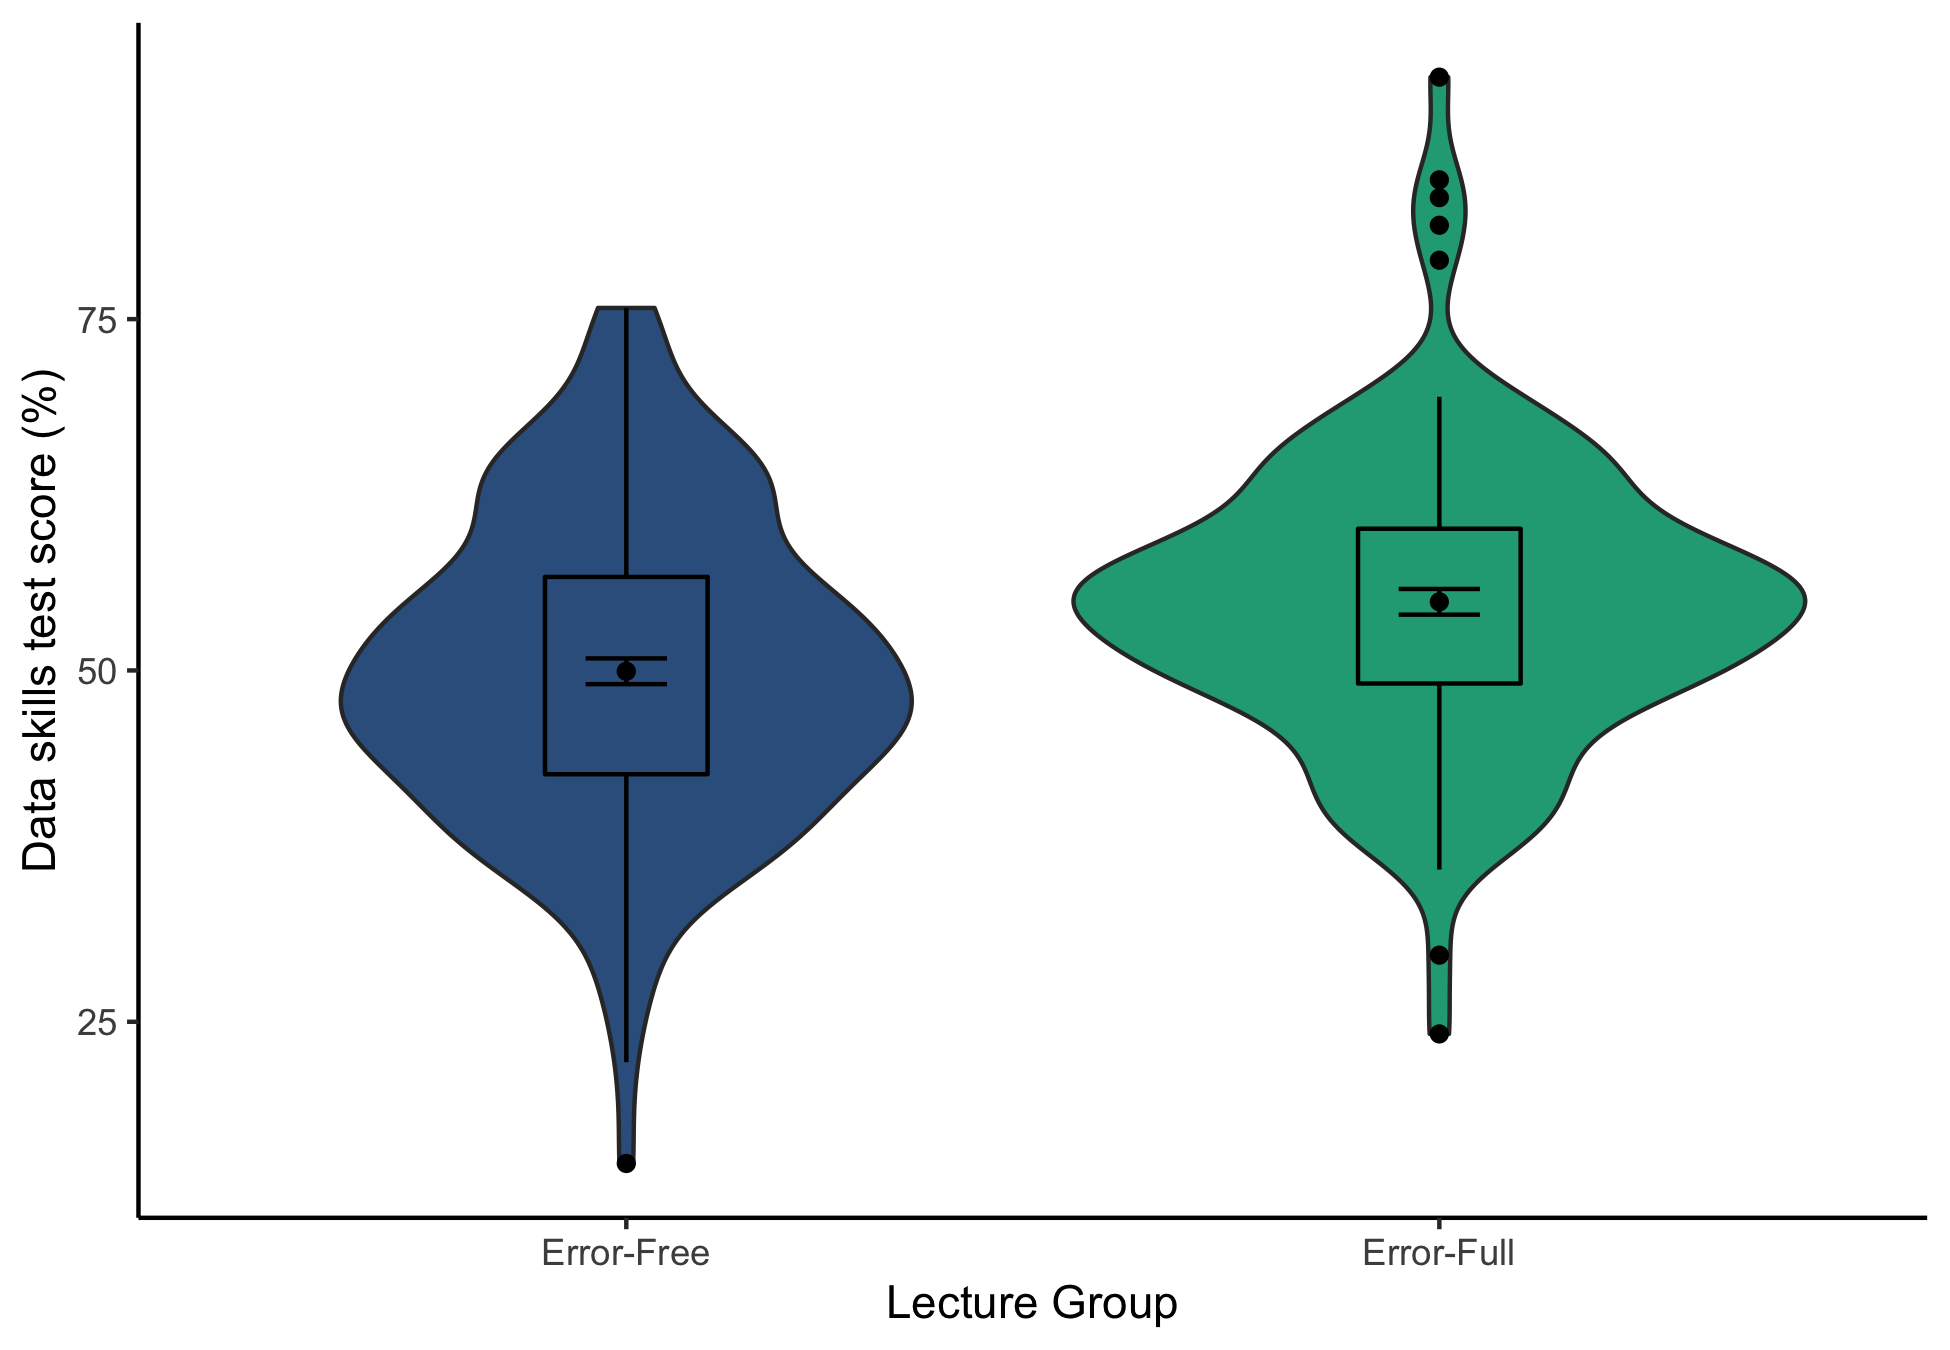
\includegraphics[width=1\linewidth]{Erroneous_code_manuscript_files/figure-latex/violin-plot-1} \caption{Violin and boxplot of the data skills assignment score for the error-free and error-full groups. The central dot shows the mean and SE instead of the median.}\label{fig:violin-plot}
\end{figure}

Consistent with our hypothesis, a Welch t-test shows that participants in the error-full group produced significantly higher data skills assignment scores than those in the error-free group, \(\Delta M = -4.94\), 95\% CI \([-7.49, -2.40]\), \(t(272.23) = -3.82\), \(p < .001\).

\hypertarget{discussion}{%
\section{Discussion}\label{discussion}}

We hypothesised that students who experienced an error-full lecture would score higher on a data skills assignment than students who experienced an error-free lecture. Consistent with our prediction, participants in the error-full group scored significantly higher than participants in the error-free group with an almost 5\% increase.

We designed our study to build on Hoffman and Elmi (2021) who compared error-full and error-free SAS lectures. However, they only recruited 18 participants in a pilot study and did not report performance data. We applied their idea to the software R and randomly allocated participants into one of two groups to evaluate the effect of this format on a data skills assignment focusing on data wrangling.

In conclusion, a lecture format that covers both data wrangling and debugging skills has the potential to improve student's understanding of reproducible data preparation and analysis.

\hypertarget{disclosures}{%
\section{Disclosures}\label{disclosures}}

We used R (Version 4.1.3; R Core Team, 2022) and the R-packages \emph{dplyr} (Version 1.0.10; Wickham, François, et al., 2022), \emph{ggplot2} (Version 3.3.6; Wickham, 2016), \emph{papaja} (Version 0.1.1; Aust \& Barth, 2022), \emph{pwr} (Version 1.3.0; Champely, 2020), \emph{readr} (Version 2.1.2; Wickham, Hester, et al., 2022), and \emph{tinylabels} (Version 0.2.3; Barth, 2022) for all our analyses.

\newpage

\hypertarget{references}{%
\section{References}\label{references}}

\hypertarget{refs}{}
\begin{CSLReferences}{1}{0}
\leavevmode\vadjust pre{\hypertarget{ref-R-papaja}{}}%
Aust, F., \& Barth, M. (2022). \emph{{papaja}: {Prepare} reproducible {APA} journal articles with {R Markdown}}. \url{https://github.com/crsh/papaja}

\leavevmode\vadjust pre{\hypertarget{ref-R-tinylabels}{}}%
Barth, M. (2022). \emph{{tinylabels}: Lightweight variable labels}. \url{https://cran.r-project.org/package=tinylabels}

\leavevmode\vadjust pre{\hypertarget{ref-bebermeier_creating_2019}{}}%
Bebermeier, S., \& Hagemann, A. (2019). Creating {Statistics} {Exercises} on the {Basis} of {Research} {Articles}. \emph{Teaching of Psychology}, \emph{46}(3), 240--245. \url{https://doi.org/10.1177/0098628319853938}

\leavevmode\vadjust pre{\hypertarget{ref-R-pwr}{}}%
Champely, S. (2020). \emph{Pwr: Basic functions for power analysis}. \url{https://CRAN.R-project.org/package=pwr}

\leavevmode\vadjust pre{\hypertarget{ref-hoffman_students_2021}{}}%
Hoffman, H. J., \& Elmi, A. F. (2021). Do {Students} {Learn} {More} from {Erroneous} {Code}? {Exploring} {Student} {Performance} and {Satisfaction} in an {Error}-{Free} {Versus} an {Error}-full {SAS}® {Programming} {Environment}. \emph{Journal of Statistics and Data Science Education}, \emph{0}(0), 1--13. \url{https://doi.org/10.1080/26939169.2021.1967229}

\leavevmode\vadjust pre{\hypertarget{ref-mcaleer_embedding_2022}{}}%
McAleer, P., Stack, N., Woods, H., DeBruine, L., Paterson, H., Nordmann, E., Kuepper-Tetzel, C. E., \& Barr, D. J. (2022). \emph{Embedding {Data} {Skills} in {Research} {Methods} {Education}: {Preparing} {Students} for {Reproducible} {Research}}. PsyArXiv. \url{https://doi.org/10.31234/osf.io/hq68s}

\leavevmode\vadjust pre{\hypertarget{ref-R-base}{}}%
R Core Team. (2022). \emph{R: A language and environment for statistical computing}. R Foundation for Statistical Computing. \url{https://www.R-project.org/}

\leavevmode\vadjust pre{\hypertarget{ref-simonsohn_small_2015}{}}%
Simonsohn, U. (2015). Small {Telescopes}: {Detectability} and the {Evaluation} of {Replication} {Results}. \emph{Psychological Science}, \emph{26}(5), 559--569. \url{https://doi.org/10.1177/0956797614567341}

\leavevmode\vadjust pre{\hypertarget{ref-targ_meta-research_group_statistics_2022}{}}%
TARG Meta-Research Group. (2022). Statistics {Education} in {Undergraduate} {Psychology}: {A} {Survey} of {UK} {Curricula}. \emph{Collabra: Psychology}, \emph{8}(1), 38037. \url{https://doi.org/10.1525/collabra.38037}

\leavevmode\vadjust pre{\hypertarget{ref-R-ggplot2}{}}%
Wickham, H. (2016). \emph{ggplot2: Elegant graphics for data analysis}. Springer-Verlag New York. \url{https://ggplot2.tidyverse.org}

\leavevmode\vadjust pre{\hypertarget{ref-R-dplyr}{}}%
Wickham, H., François, R., Henry, L., \& Müller, K. (2022). \emph{Dplyr: A grammar of data manipulation}. \url{https://CRAN.R-project.org/package=dplyr}

\leavevmode\vadjust pre{\hypertarget{ref-R-readr}{}}%
Wickham, H., Hester, J., \& Bryan, J. (2022). \emph{Readr: Read rectangular text data}. \url{https://CRAN.R-project.org/package=readr}

\end{CSLReferences}


\end{document}
